\section{Detector performance}

In order to calibrate detectors and test their performances, a cosmic test bench was designed and installed at Saclay 
early in the project (Figure \ref{fig:mm-testbench}). The goal of these tests is to determine the best operating 
conditions of a detector and to compute its 2D efficiency map using cosmic muons prior shipment to Jefferson Lab.


\begin{figure}[htb]
 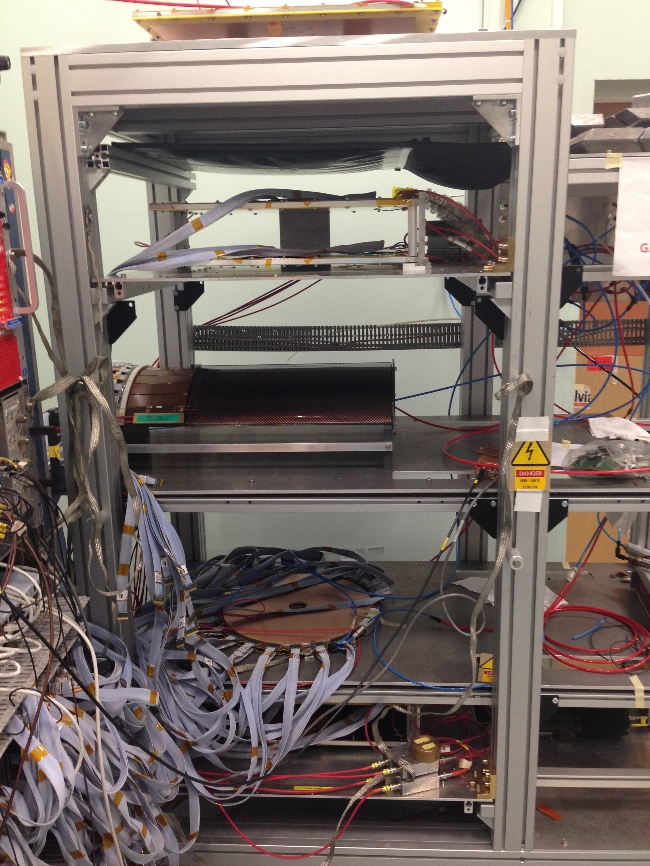
\includegraphics[width=1.0\columnwidth,keepaspectratio]{images/banc_cosmique}
 \caption{Cosmic bench made of an external trigger from the coincidence of two scintillators and a hodoscope made of 4 
reference trackers. The picture shows the operation of a Barrel and a Forward detector simultaneously under test.}
 \label{fig:mm-testbench}
\end{figure}

The cosmic test bench shown on Figure~\ref{fig:mm-testbench}, consists of a vertical stack of six detectors. Two scintillators are installed 
at the top and the bottom of the stack to provide the trigger. Four $50 \times 50 \text{ cm}^2$ double-layers flat 
Micromegas are used as a tracker to provide the reference track of a cosmic ray. In the middle of the stack, empty 
trays receive the detectors to be characterized.

After alignment of the reference trackers and the detectors in test, an expected position of the particle in the detector in test is provided by the reference and compared with measured signals, if any, in the detector to be tested. If a signal matches the expected position within a millimeter, the detector in test is considered to have seen the cosmic rays. An efficiency is then derived by repeating this test over a cosmic ray sample collected within a few hours. All MVT detectors have been systematically characterized before shipment to JLab. These tests included a study of the efficiency as a 
function of the amplification voltage and a two-dimensional efficiency map which requires a cosmic ray sample collected over a day.

The results were found similar for all detectors: the efficiency plateau starts at about 500V with a value between 98.5\% and 
99.5\% at 510V. It was shown that the plateau was slightly shifted to higher strip voltages when the drift plane is at 
higher voltage because the mesh loses electron transparency. The 2D-efficiency map was useful to look for any 
structural problem. All MVT detectors that were shipped to Jefferson Lab had uniform 2D-efficiency map. An example of 
the efficiency plateau and the 2D efficiency map is shown in Figure \ref{fig:mm-fig8} and \ref{fig:mm-fig9}. Figure \ref{fig:mm-fig9} shows the efficiency gain by removing the protection diodes in front of the front-end chip "DREAM". Since we are using the resisitive Micromegas technology, sparks are quenched and protection of the front-end electronics is no longer required (beside the chip packaging protection) even with high gain in beam condition.

\begin{figure}[htb]
 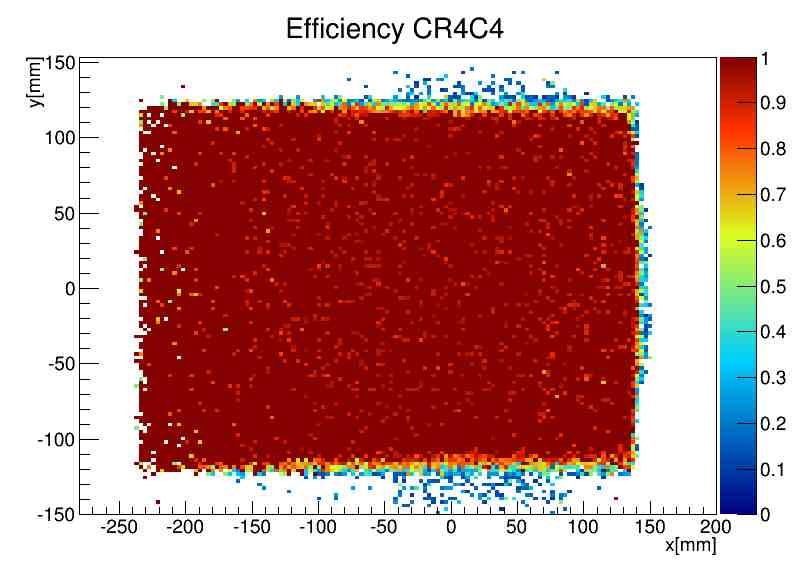
\includegraphics[width=1.0\columnwidth,keepaspectratio]{images/Eff_2D}
 
 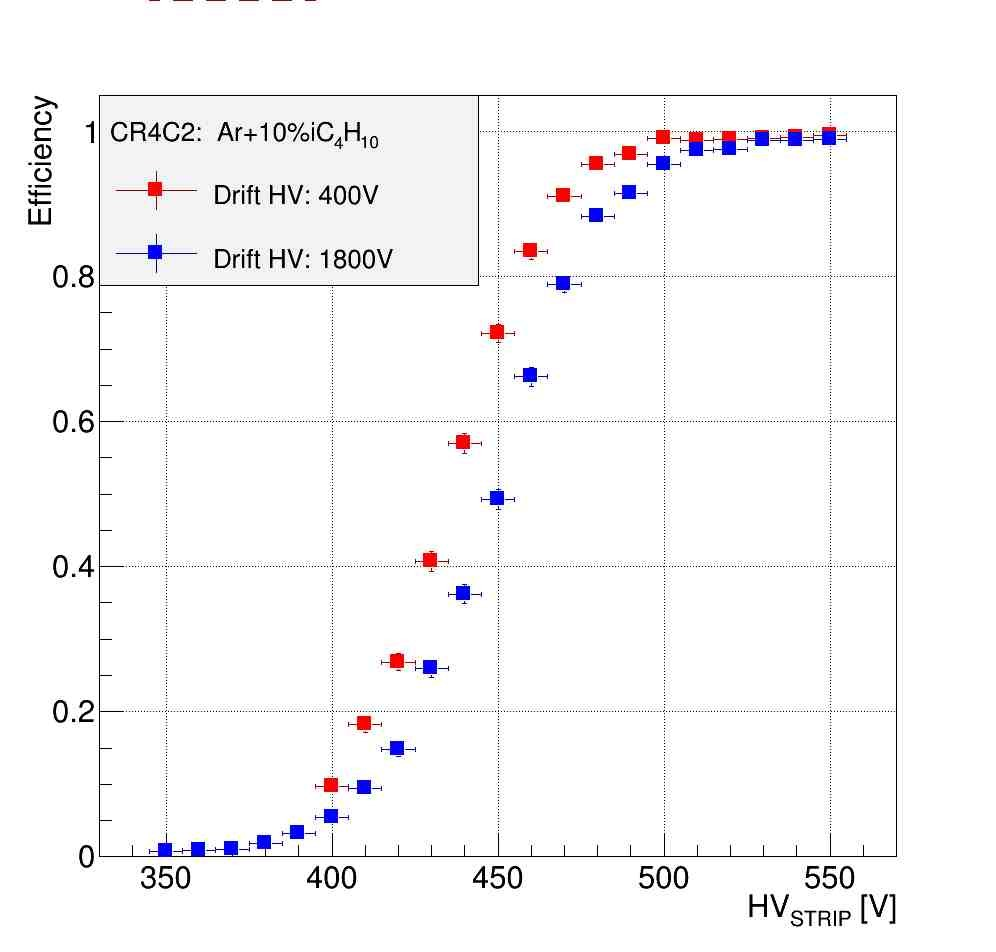
\includegraphics[width=1.0\columnwidth,keepaspectratio]{images/Plateau_HV}
 
 \caption{Efficiency plateau (bottom) and 2D map (top) for a C-type barrel detector.}
 \label{fig:mm-fig8}
\end{figure}


\begin{figure}[htb]
 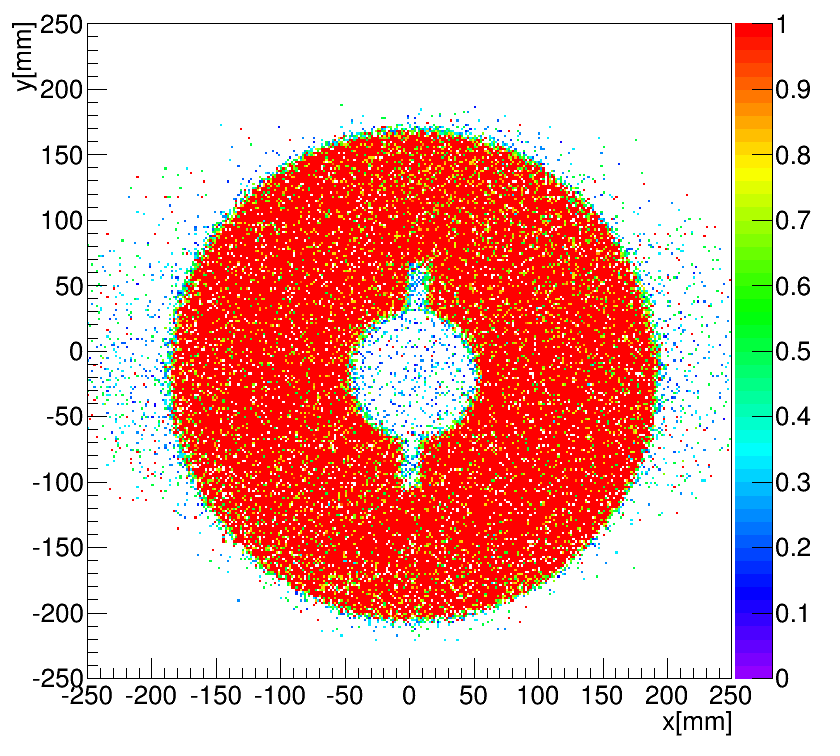
\includegraphics[width=1.0\columnwidth,keepaspectratio]{images/FMT_eff_2Dmap_testBench.png}
 
 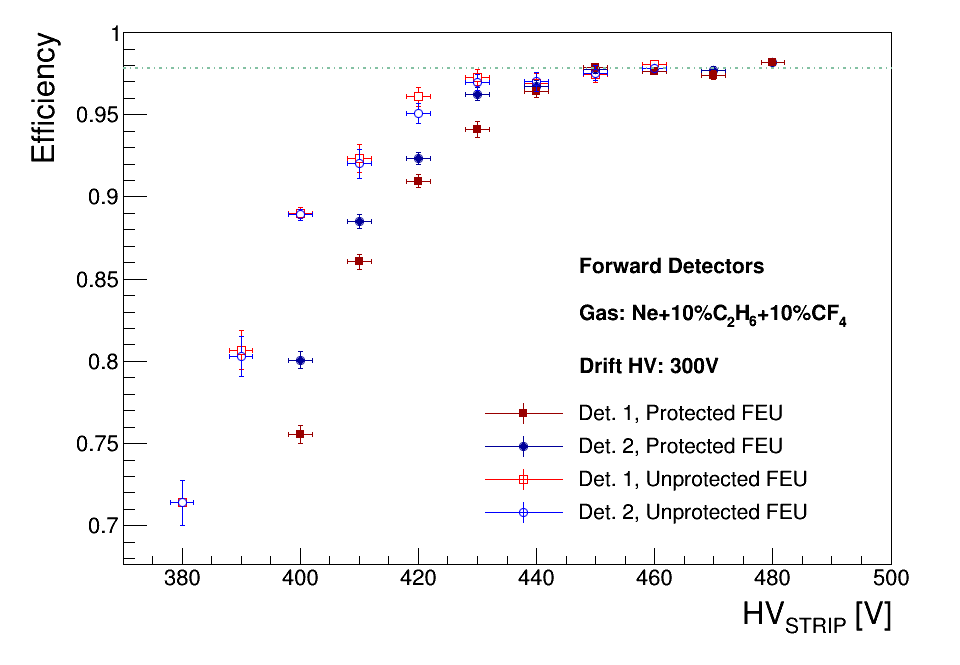
\includegraphics[width=1.0\columnwidth,keepaspectratio]{images/FMT_eff_plateau_testBench.png}
 
 \caption{Efficiency plateau (bottom) and 2D map (top) for a FMT disk.}
 \label{fig:mm-fig9}
\end{figure}

\subsection{Commissioning}

The Micromegas vertex tracker was delivered in June 2017 at Jefferson Laboratory. A team of 10 people assembled the MVT and integrated it with the SVT to form the final configuration of the CLAS12 central vertex tracker.  The MVT barrel was first commissioned with cosmic rays in a gray room until mid-October and for the first two weeks once installed in the Hall. The final phase of the commissioning started in December 2017 with beam.

Before the start of the data taking with beam, several cosmic rays data taking runs have been performed with the aim at tuning and optimizing the integration of the data acquisition system, the slow-control (i.e. remote controls, interlocks and monitoring) and the gas delivery system. The online data monitoring system was developed to allow the inspection of raw quantities such as the hit maps, the pulse shape and the timing of the signals. It was tested and integrated into the CLAS12 operation tools. 

\subsection{Cosmic rays data taking}

Cosmic rays data with zero magnetic field have been used not only for commissioning purposes, but they result essential for the detector alignment.

Given the absence of the solenoid magnetic field, the drift high voltages are set to about 400V as the primary electrons do not experience the Lorentz-angle effect. The cosmic rays trigger for the central detectors is provided by coincidences of CTOF signals in rather diametrically opposed scintillator bars. This CTOF trigger provides provides a quasi-uniform illumination along the BMT axis of the barrel with cosmic rays, not achievable in beam condition because of the forward boost. The hit distribution on the Z-tiles, instead, results from a convolution of the cosmic rays angular distribution with the trigger configuration. As it is shown in Figure~\ref{fig:mm-cosmic_occupancy}, the sector 2 has about twice as many hits as sector 1 and 3 since it is at the top of the barrel and cosmics comes from the sky. The trigger requiring signals in rather diametrically opposed scintillator bars, the dip of occupancy in sector 1 and 3 is explained by the horizontal muon flux being very low.

\begin{figure}[htb]
 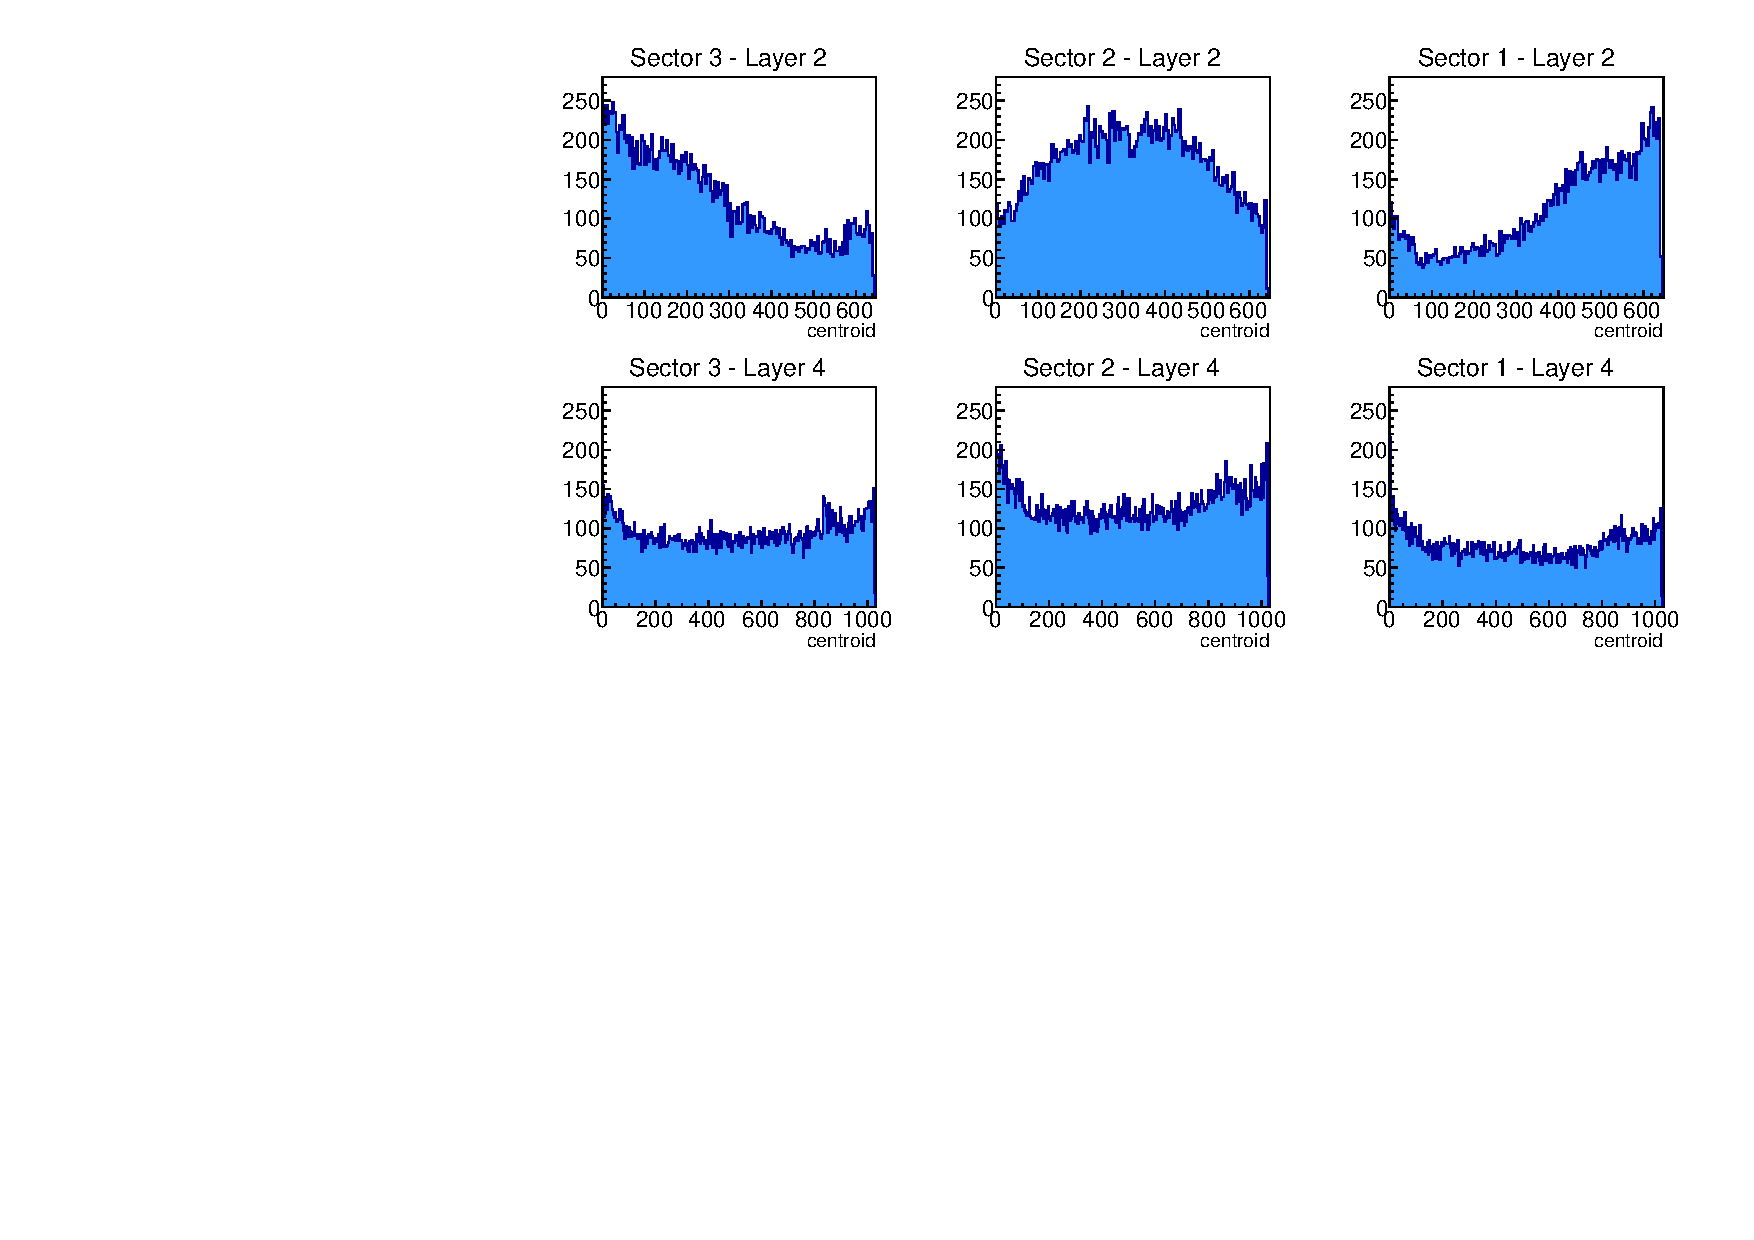
\includegraphics[width=.45\textwidth]{images/BMT_hit_cosmics_CTOFtrigger.pdf}
 \caption{Hit occupancies of a cosmic-ray run with the trigger delivered by the CTOF for the layers 3 (Z-tile) and 4 (C-tile).}
 \label{fig:mm-cosmic_occupancy}
\end{figure}

The distributions of cluster size for the three sectors, Figure~\ref{fig:mm-cosmic_cls}, show a higher probability in sector 1 and 3 for larger cluster size values. Indeed, since cosmic rays are mostly vertical, the projection of their path in the drift gap onto the strip surface is longer for sectors 1 and 3 than in sector 2.

\begin{figure}[htb]
 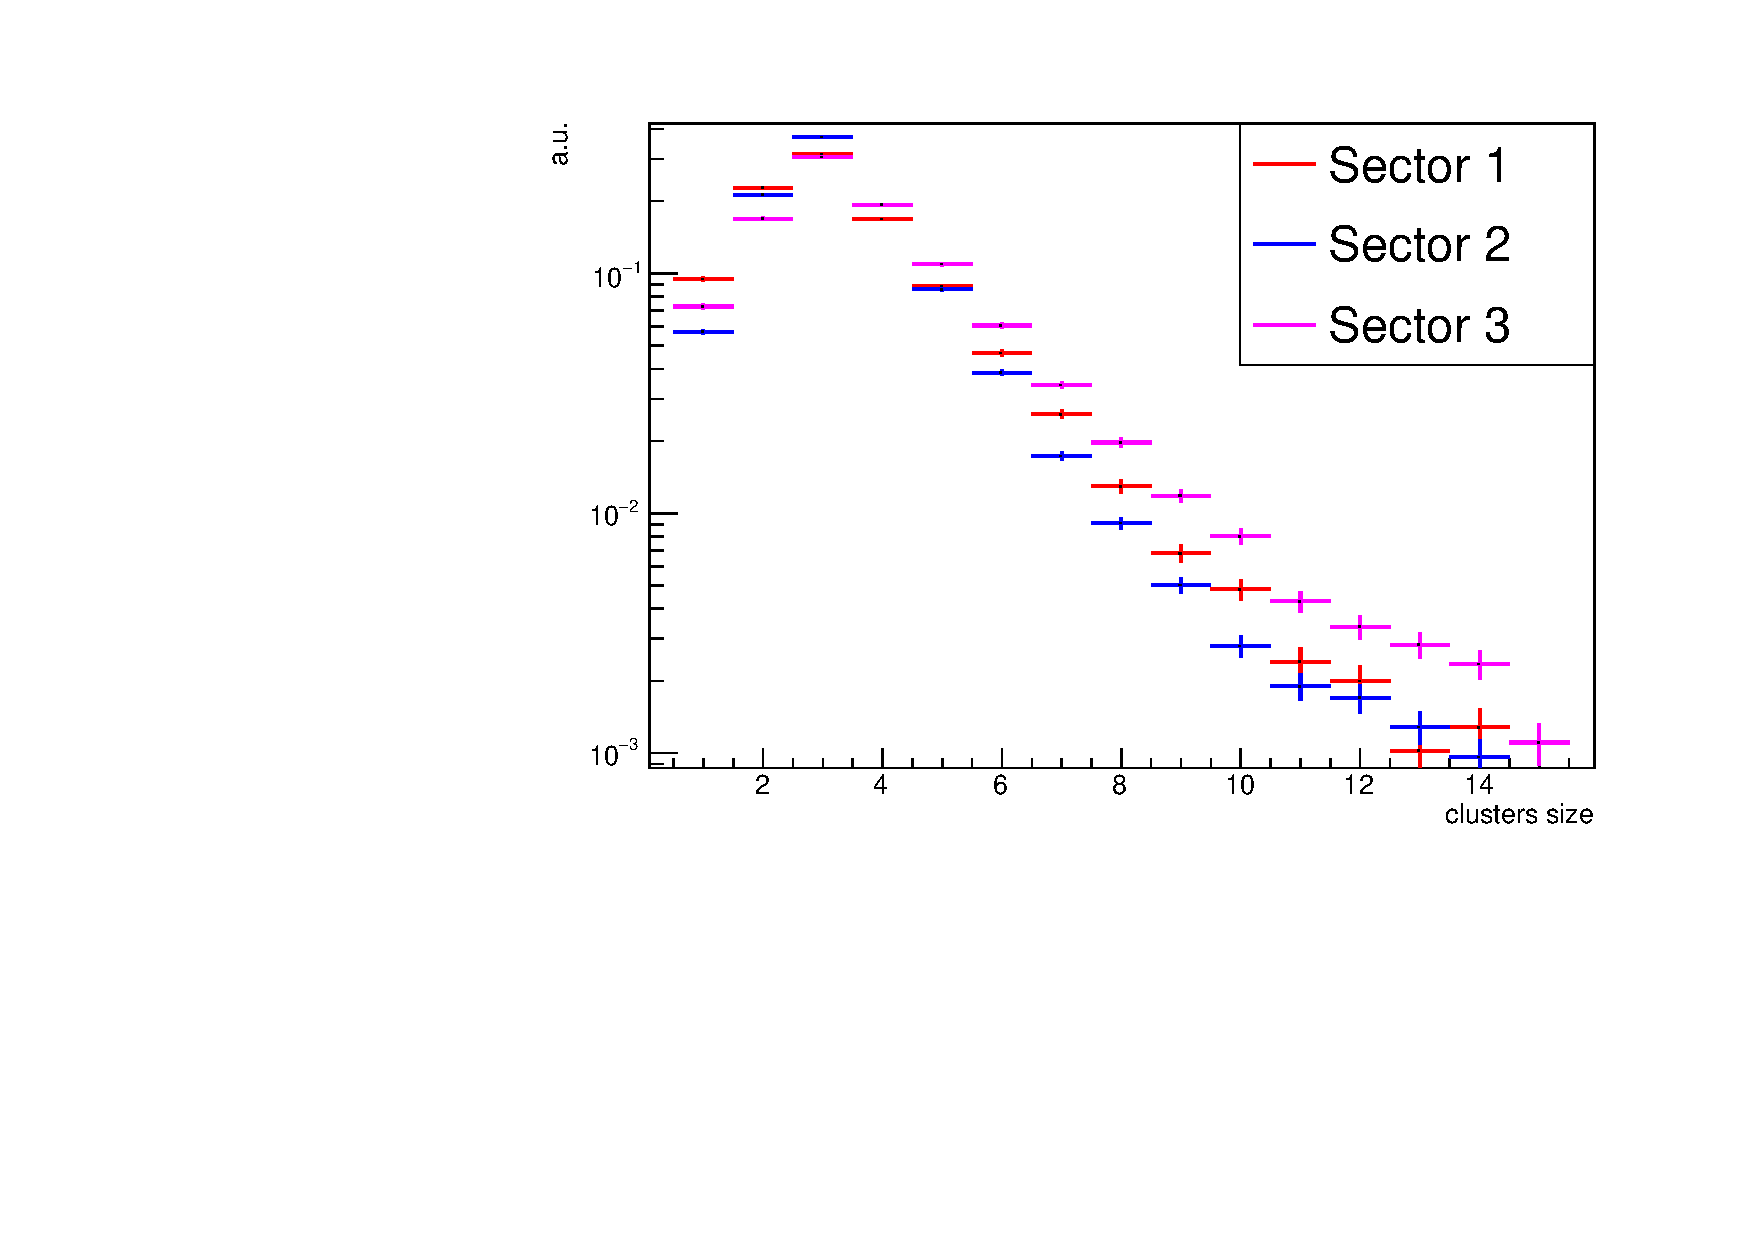
\includegraphics[width=.45\textwidth]{images/cosmic_cluster_size.pdf}
 \caption{Cluster size distributions during cosmic ray data taking for the three sectors.}
 \label{fig:mm-cosmic_cls}
\end{figure}

A BMT standalone straight-track algorithm based on least-square minimization has been developed to reconstruct cosmic ray tracks. A typical reconstructed event is shown in Figure~\ref{fig:mm-cosmic_ced} using the Clas12 event display package \cite{nim:rec-ced}.
This tracking algorithm is also used to perform the alignment of the BMT tiles: the distance between the hit in a tile excluded from the tracking and the reference track provided by the other tiles is minimized by introducing rotations and translations. Figure~\ref{fig:mm-cosmic_residuals} shows distributions of track residuals, i.e. the distance of a hit with respect to the particle trajectory, for three Micromegas tiles before and after alignment corrections. Figure~\ref{fig:mm-cosmic_res_summary} shows the summary of the preliminary results for all the BMT detectors: after the alignment procedure all residual distributions are centered around zero. Preliminary detector resolutions obtained from the standard deviations of the residual distributions are improved and below 200$\mu$m. 

\begin{figure}[htb]
 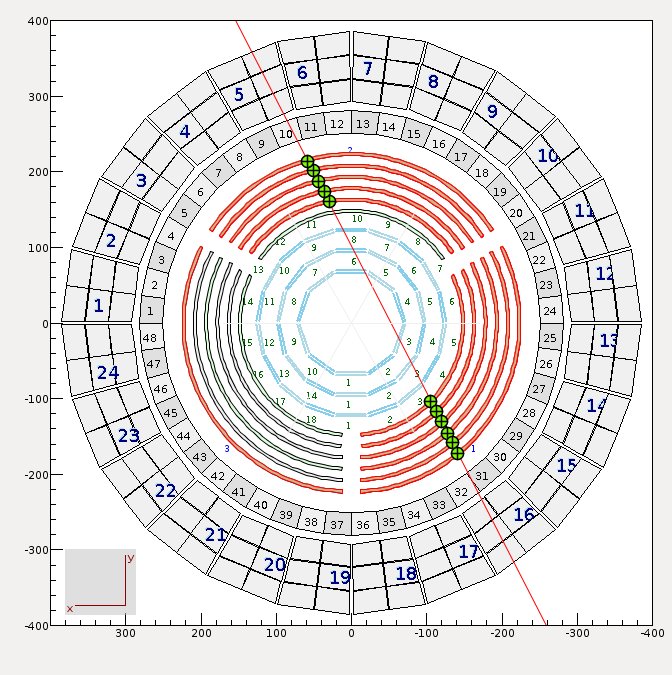
\includegraphics[width=.4\textwidth]{images/cosmic_NIM.png}
 \caption{Event display of a cosmic ray track reconstructed in the BMT detectors.}
 \label{fig:mm-cosmic_ced}
\end{figure}

\begin{figure}[htb]
 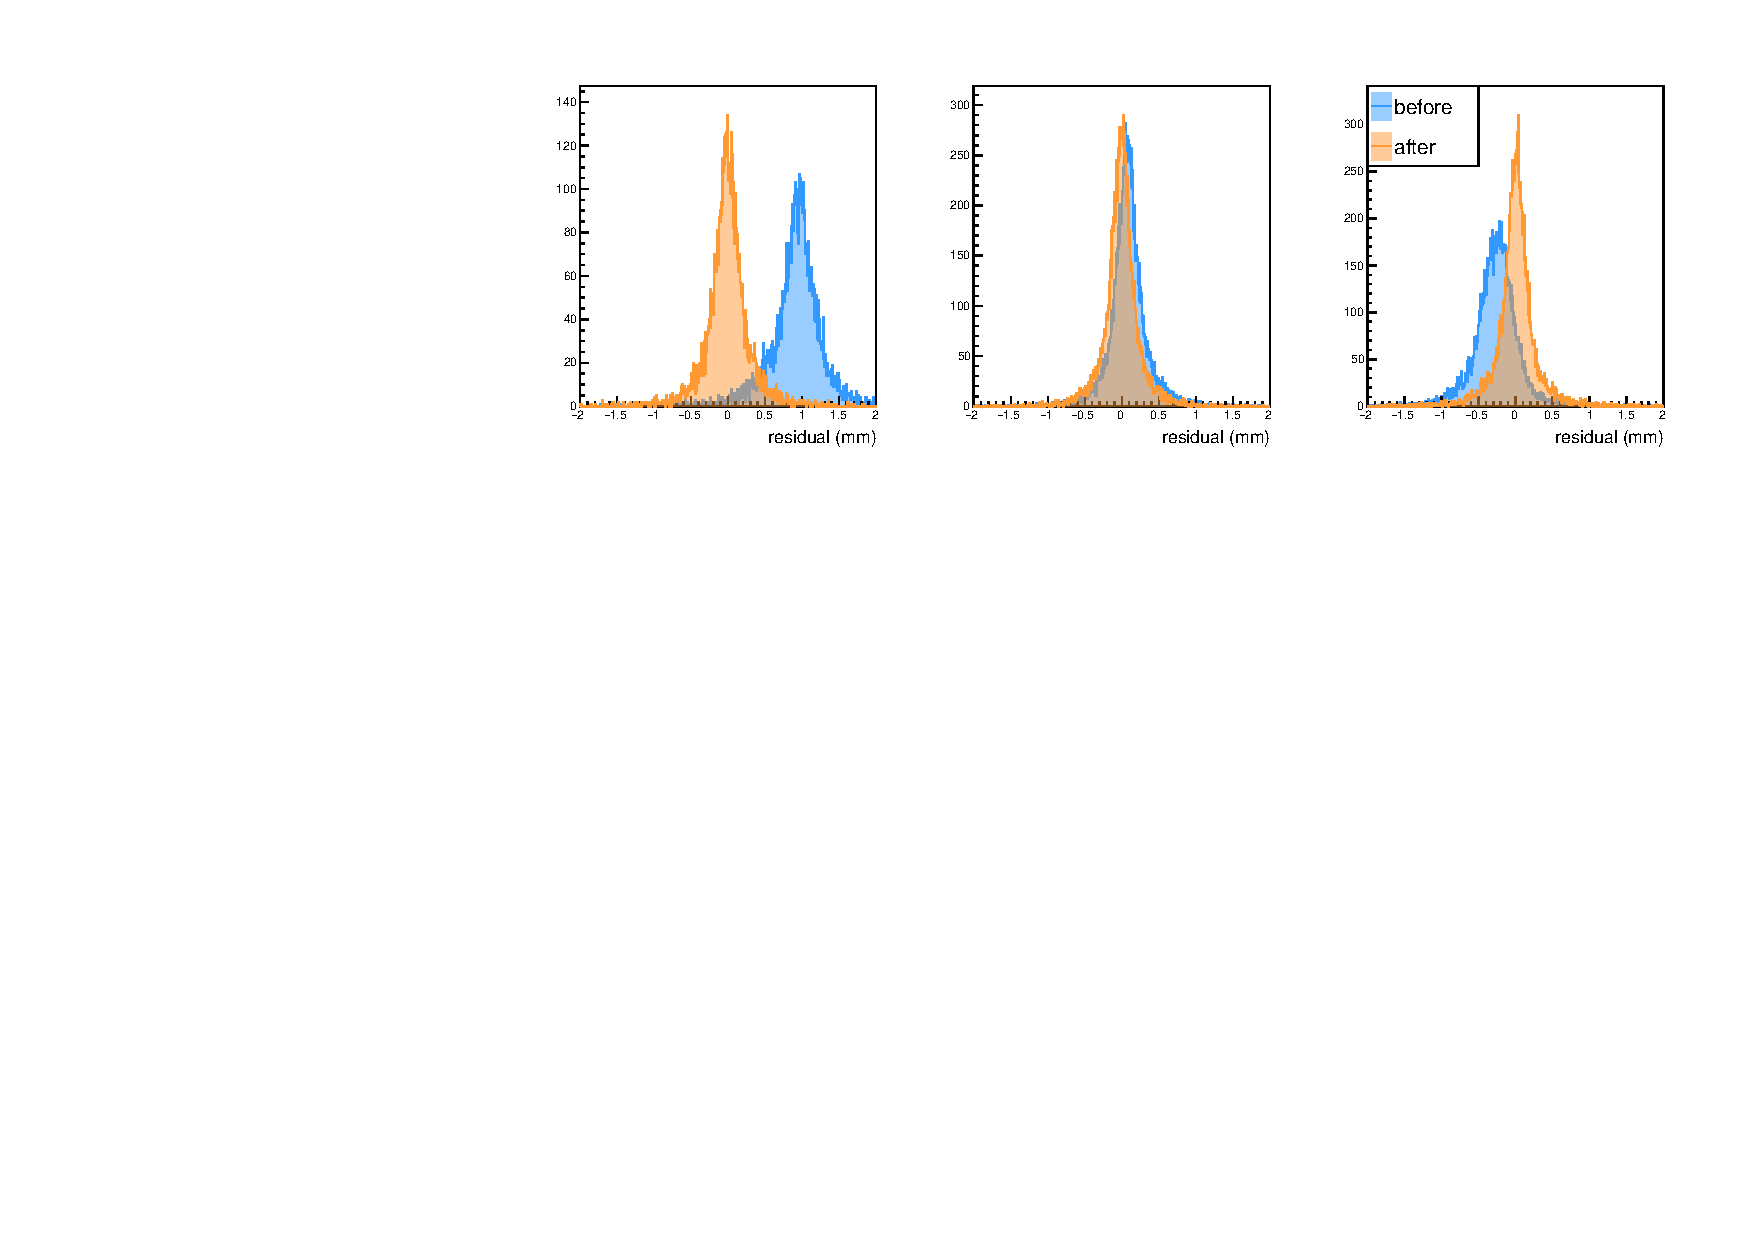
\includegraphics[width=.45\textwidth]{images/cosmic_residuals.pdf}
 \caption{Example of BMT residuals with cosmic ray data before and after a preliminary alignment procedure obtained with a BMT standalone reconstruction.}
 \label{fig:mm-cosmic_residuals}
\end{figure}

\begin{figure}[htb]
 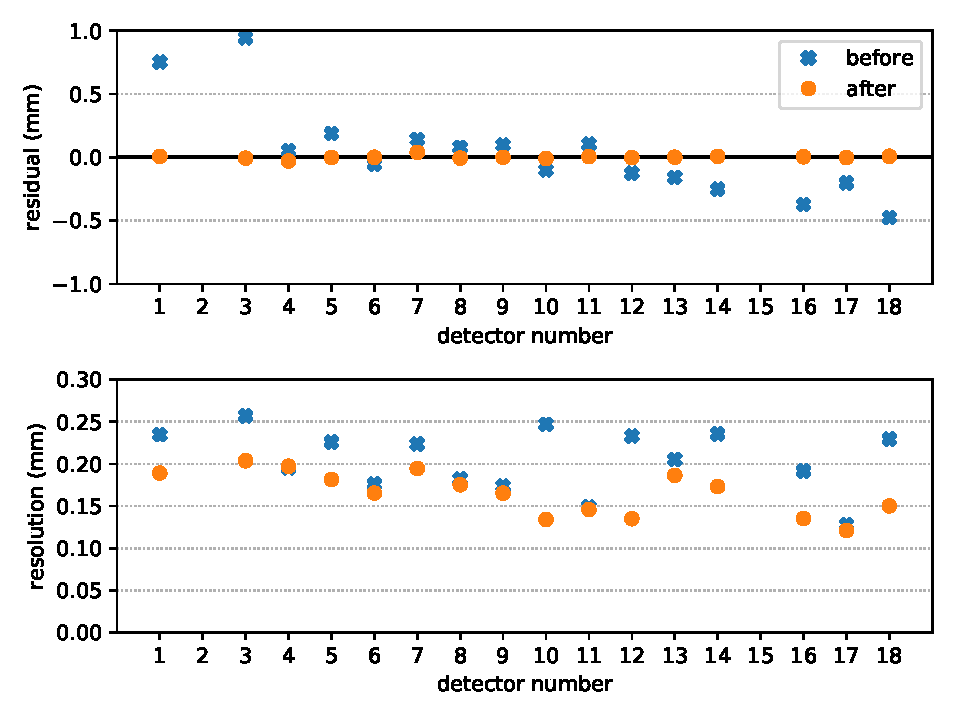
\includegraphics[width=\columnwidth]{images/residuals_and_resolutions.pdf}
 \caption{Preliminary BMT residuals with cosmic ray data before and after an alignment procedure obtained with a BMT standalone reconstruction.}
 \label{fig:mm-cosmic_res_summary}
\end{figure}

\subsection{Data taking with beam}

With the start of the operations with beam, the behaviour of the detectors have been carefully monitored and the working parameters such as high voltage settings have been tuned.

The working point for the strip high voltage has been studied by performing a scan with a 20V-step. Due to the delays in the offline data reconstruction for a proper efficiency measurement, the cluster multiplicity per electron trigger was instead used as an alternative observable accessible online which may exhibit a plateau. 
Indeed, as shown on Figure \ref{fig:mm-fig15}, this observable was found to get flatter where the efficiency plateau was expected to be from the commissioning with cosmic rays.  For the FMT, the plateau was found from 460V to 490V. Above 490V, the cluster multiplicity and the current on the strips increase suddenly, potentially due to a Corona effect. It was decided to set 460V as nominal HV settings for FMT, which allows safe operations at nominal luminosity. The nominal HV setting was decided to be 520V for BMT although the plateau was not as clear as for the FMT.  

\begin{figure}[htb]
 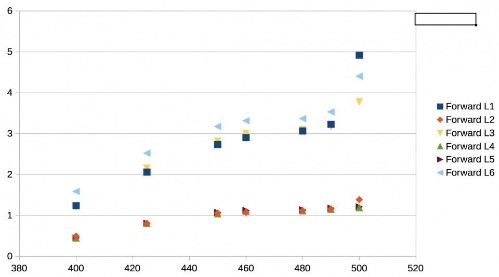
\includegraphics[width=1.0\columnwidth,keepaspectratio]{images/Plateau_cluster_FMT.jpg}
 \caption{Cluster multiplicity in FMT as a function of HV on the strips.}
 \label{fig:mm-fig15}
\end{figure}

Preliminaries efficiencies were derived once the offline reconstruction was performed. For the efficiency determination, the hits of the BMT tile under study are removed from the track searching patter recognition algorithm and, once a track is found, the tile is considered efficient if a hit is found close to the intersection of the track with the detector. All data files from the HV scan have been reconstructed and the efficiency plateau has been found for each tile at the same setting as indicated by the cluster multiplicity plateau. An example of the efficiency HV scan for one BMT detector is shown in Figure \ref{fig:mm-eff_scan}.

\begin{figure}[htb]
 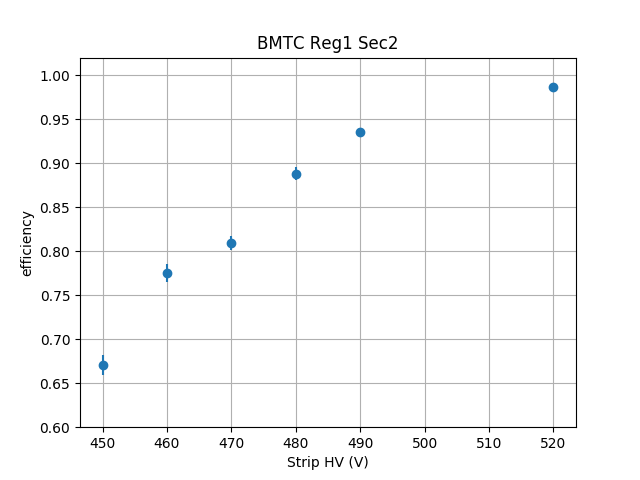
\includegraphics[width=1.0\columnwidth,keepaspectratio]{images/hvscan_BMTC_R1_S2.png}
 \caption{Efficiency measurement as a function of the strip high voltage for one tile in beam condition.}
 \label{fig:mm-eff_scan}
\end{figure}

During a beam intensity scan up to the instantaneous luminosity of about $10^{35}$Hz~cm${-2}$, the strip currents and the detector occupancy have been measured. Figure~\ref{fig:mm-fig14} shows the positive correlation between the currents drawn by the BMT strips and the beam current. The slope coefficient resulting from a linear regression is $0.02~\mu\text{A}/n\text{A}$. At the maximum beam current of 78 nA, two BMT tiles reached the safety threshold of 2 $\mu$A and they were automatically turned off. The detector occupancy shows as well a linear correlation with the beam current, reaching values of about 3.5\% for the FMT disks and 2.5\% for the BMT tiles at nominal luminosity, as shown on Figure~n\ref{fig:mm-fig16}.

\begin{figure}[htb]
 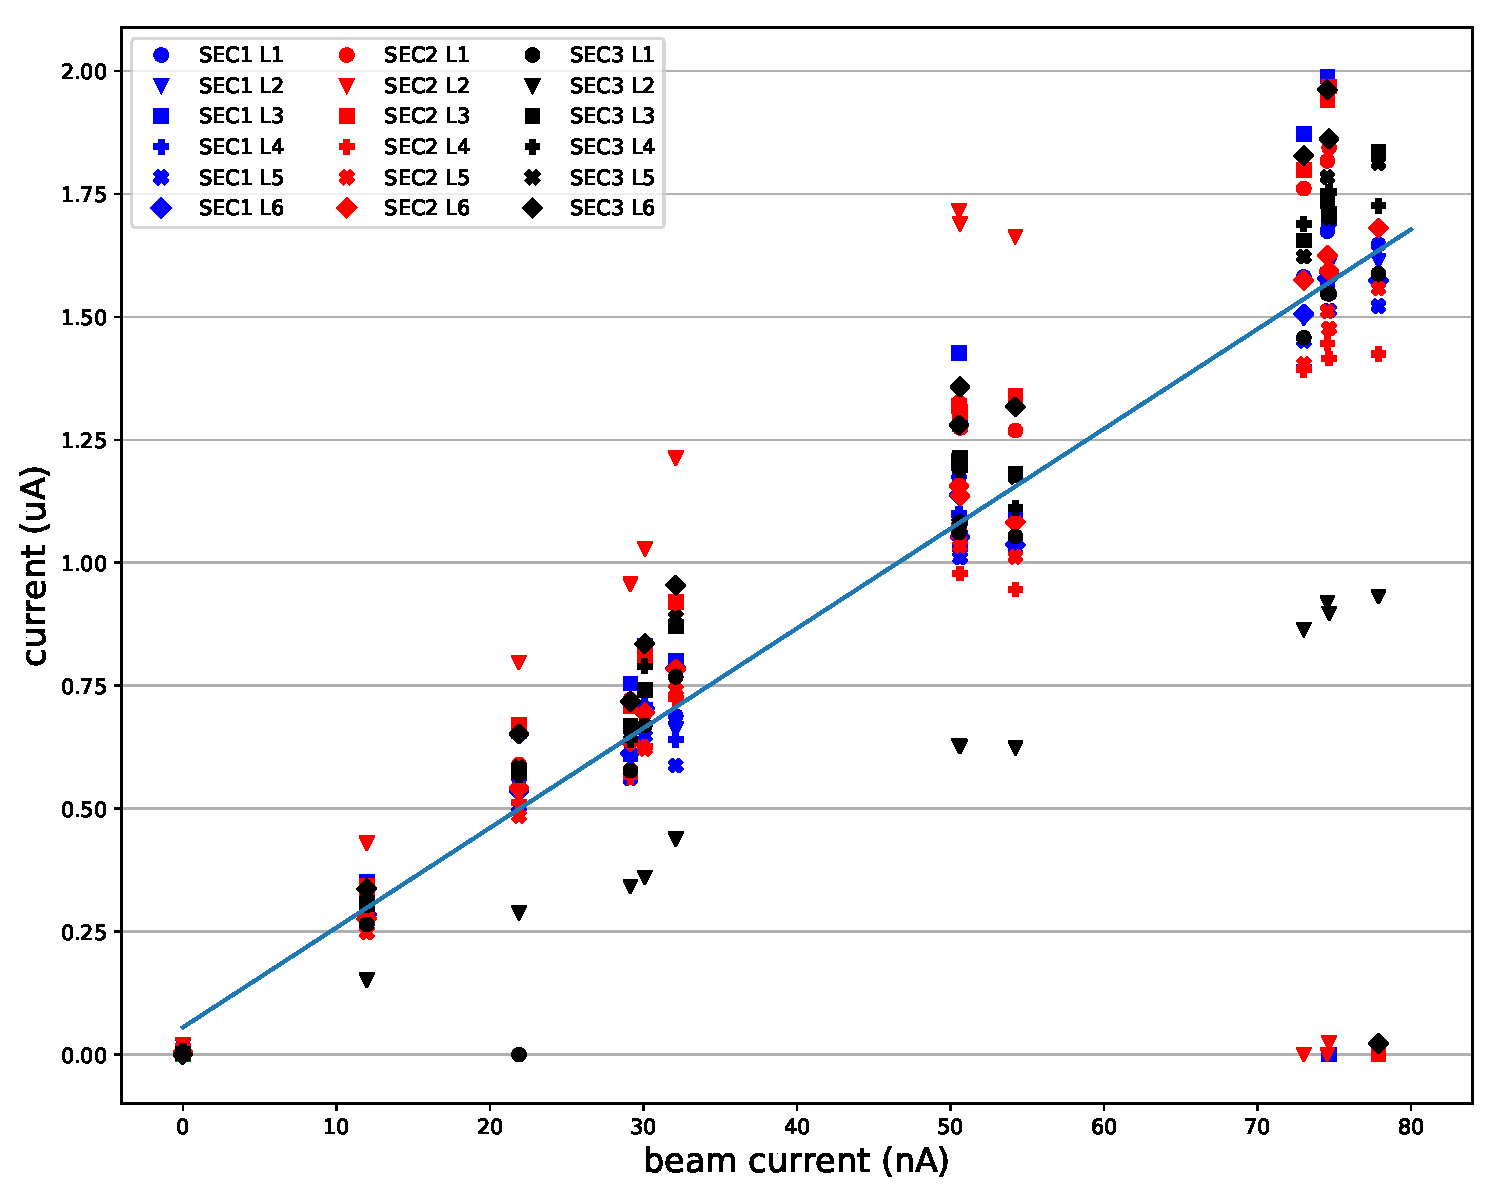
\includegraphics[width=1.0\columnwidth,keepaspectratio]{images/BMT_IvsLumi}
 \caption{Currents on the strips as a function of beam current on full 5cm-long liquid H$_2$ target. All detectors have similar currents. The nominal luminosity of $10^{35}\text{cm}^{-2}\text{s}^{-1}$ corresponds to 75~nA on 5cm-long LH2 target.}
 \label{fig:mm-fig14}
\end{figure}



\begin{figure}[htb]
 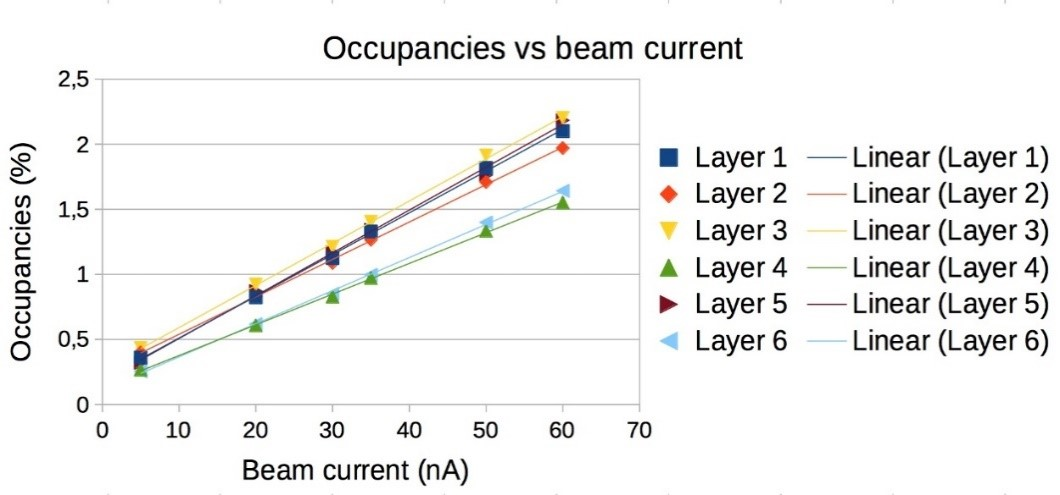
\includegraphics[width=1.0\columnwidth,keepaspectratio]{images/BMT_occ_beam.jpg}
 
 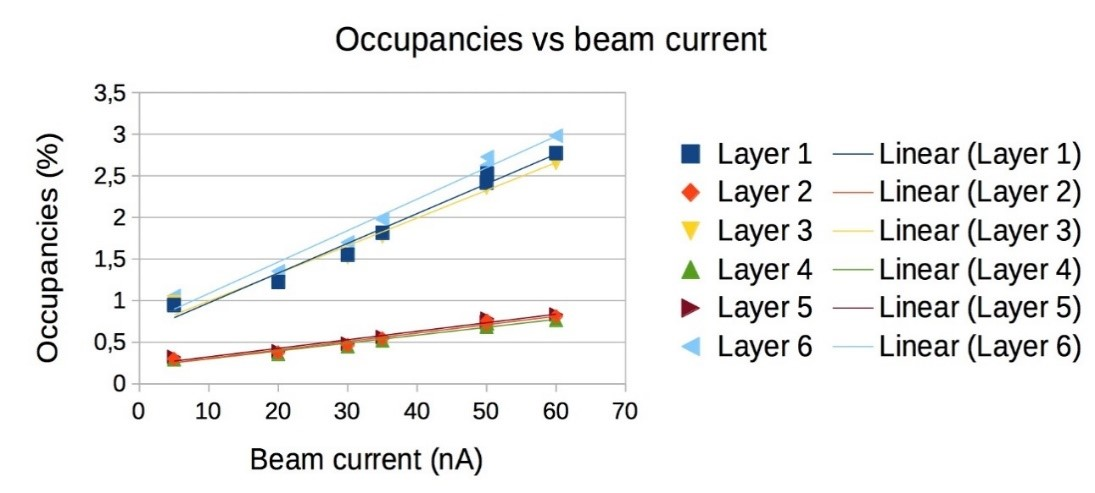
\includegraphics[width=1.0\columnwidth,keepaspectratio]{images/FMT_occ_beam.jpg}
 \caption{BMT (top) and FMT (bottom) hit occupancy as a function of the beam current.}
 \label{fig:mm-fig16}
\end{figure}


During the first year of operations with beam, CLAS12 took data at several electron beam energies (2.2, 6,4, 7.8 and 10.6 GeV) with an liquid hydrogen target. At 2.2~GeV, the large elastic cross-section and the trigger configuration allows to visualize the recoil protons in the raw occupancies of BMT-C tiles as seen in Figure~\ref{fig:mm-occupancy_22_10}. 

\begin{figure}[htb]
 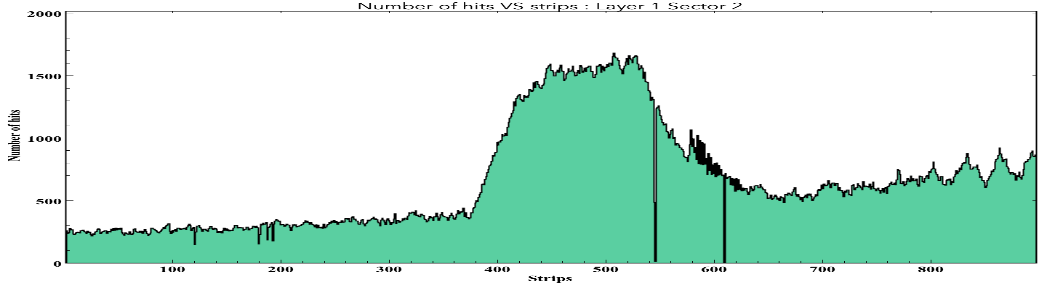
\includegraphics[width=1.0\columnwidth,keepaspectratio]{images/occupancy2GeV.png}
 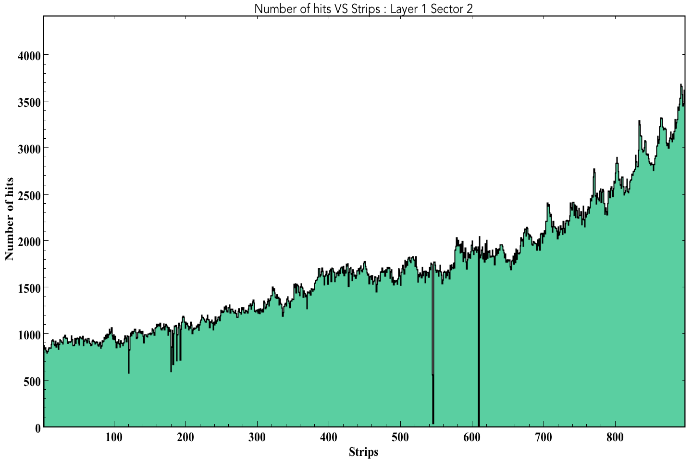
\includegraphics[width=1.0\columnwidth,height=0.3\columnwidth]{images/occupancy10GeV.png}
 \caption{Hit occupancy for C-tiles at 2.2 GeV (top) and 10.6 (bottom) in events triggered by an electron in the forward CLAS12 detectors. The elastic recoil protons are responsible for the large excess of events at 2.2 GeV, between strip number 400 and 500. At 10.6 GeV, the elastic cross sections is too small and no protons excess is visible.  }
 \label{fig:mm-occupancy_22_10}
\end{figure}

The largest data set has been collected with at the electron beam energy of 10.6~GeV and at 50~nA intensity. Figure~\ref{fig:mm-beam_cls} shows the distributions of the number of clusters on all the six BMT layers and their cluster size distribution. Although most of the events present a very low number of clusters with clusters of small size, the long tails are mainly due to knock-off electron loopers and beam induced soft photons.

\begin{figure}[htb]
 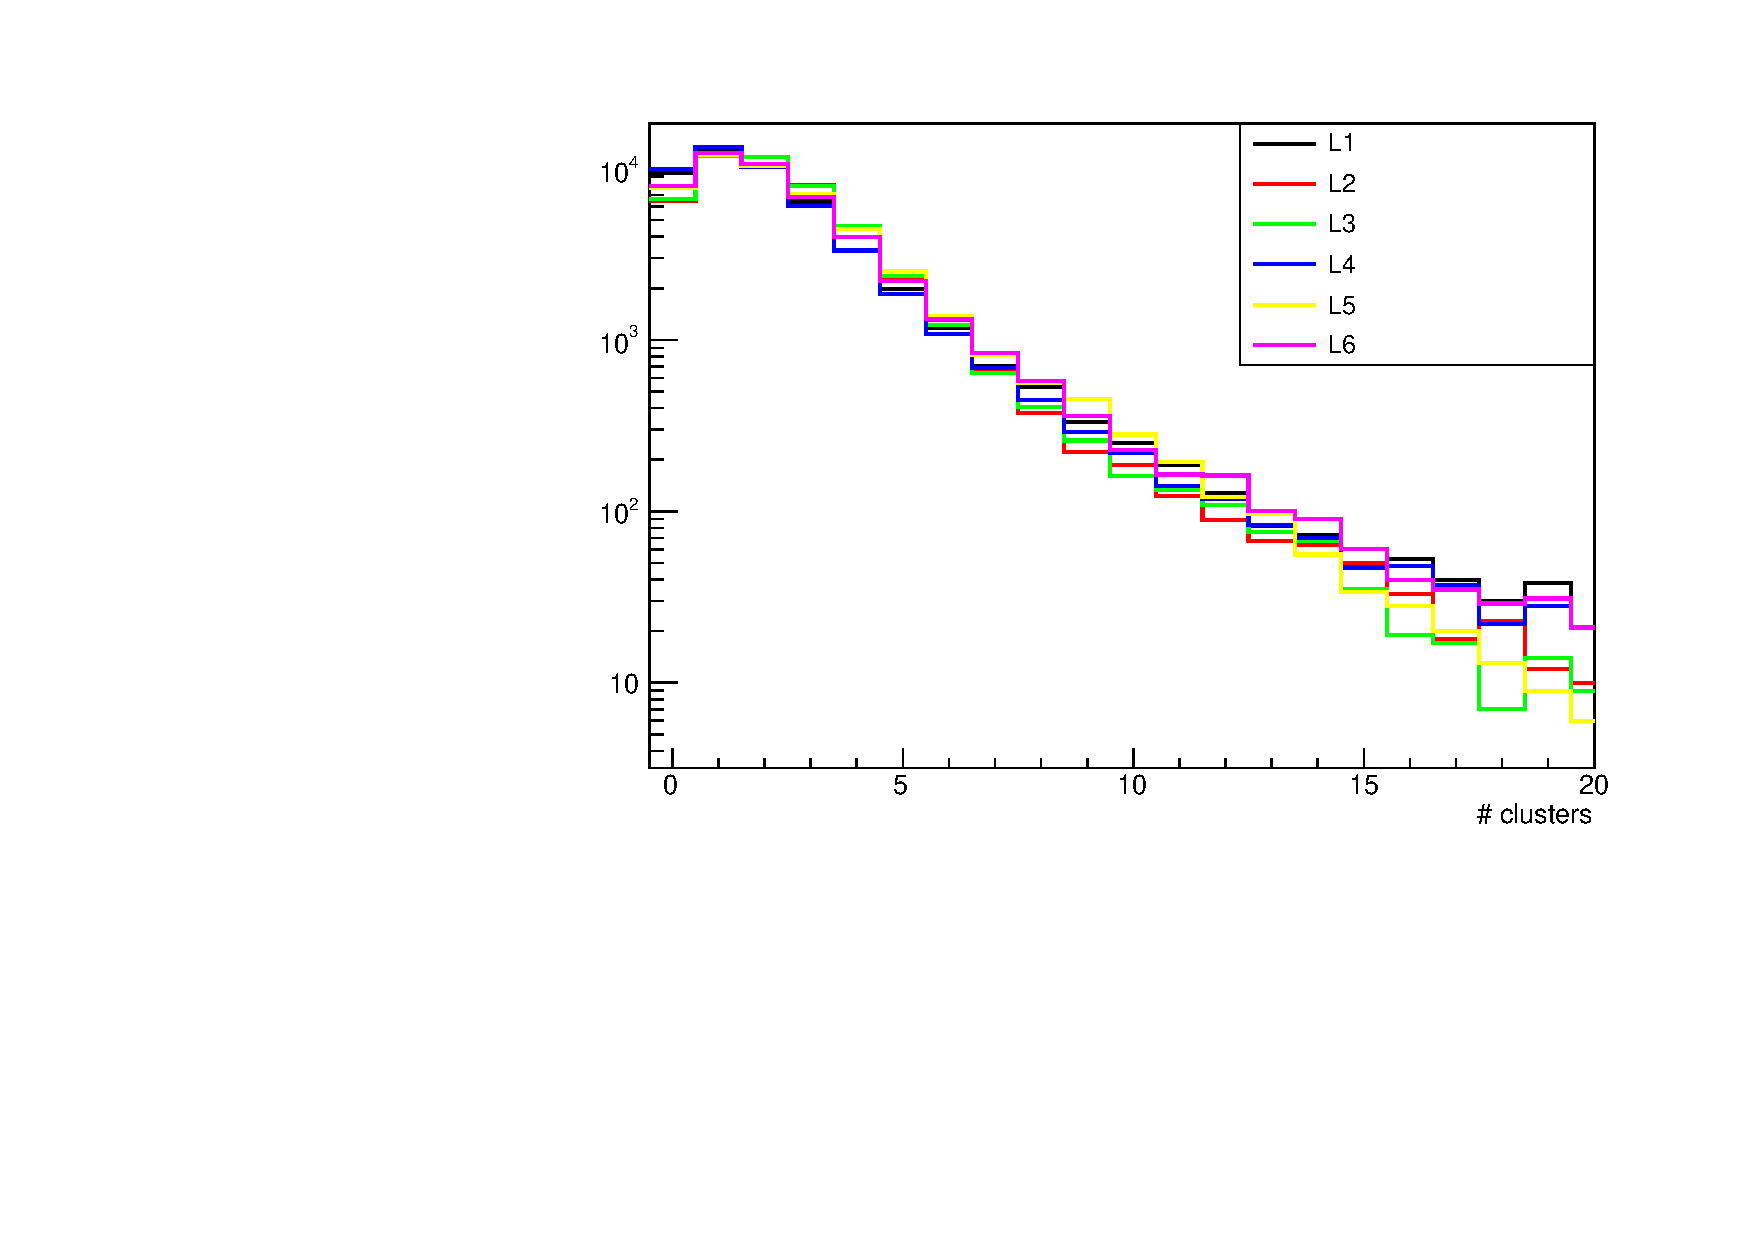
\includegraphics[width=.49\columnwidth,keepaspectratio]{images/beam_num_cls.pdf}
 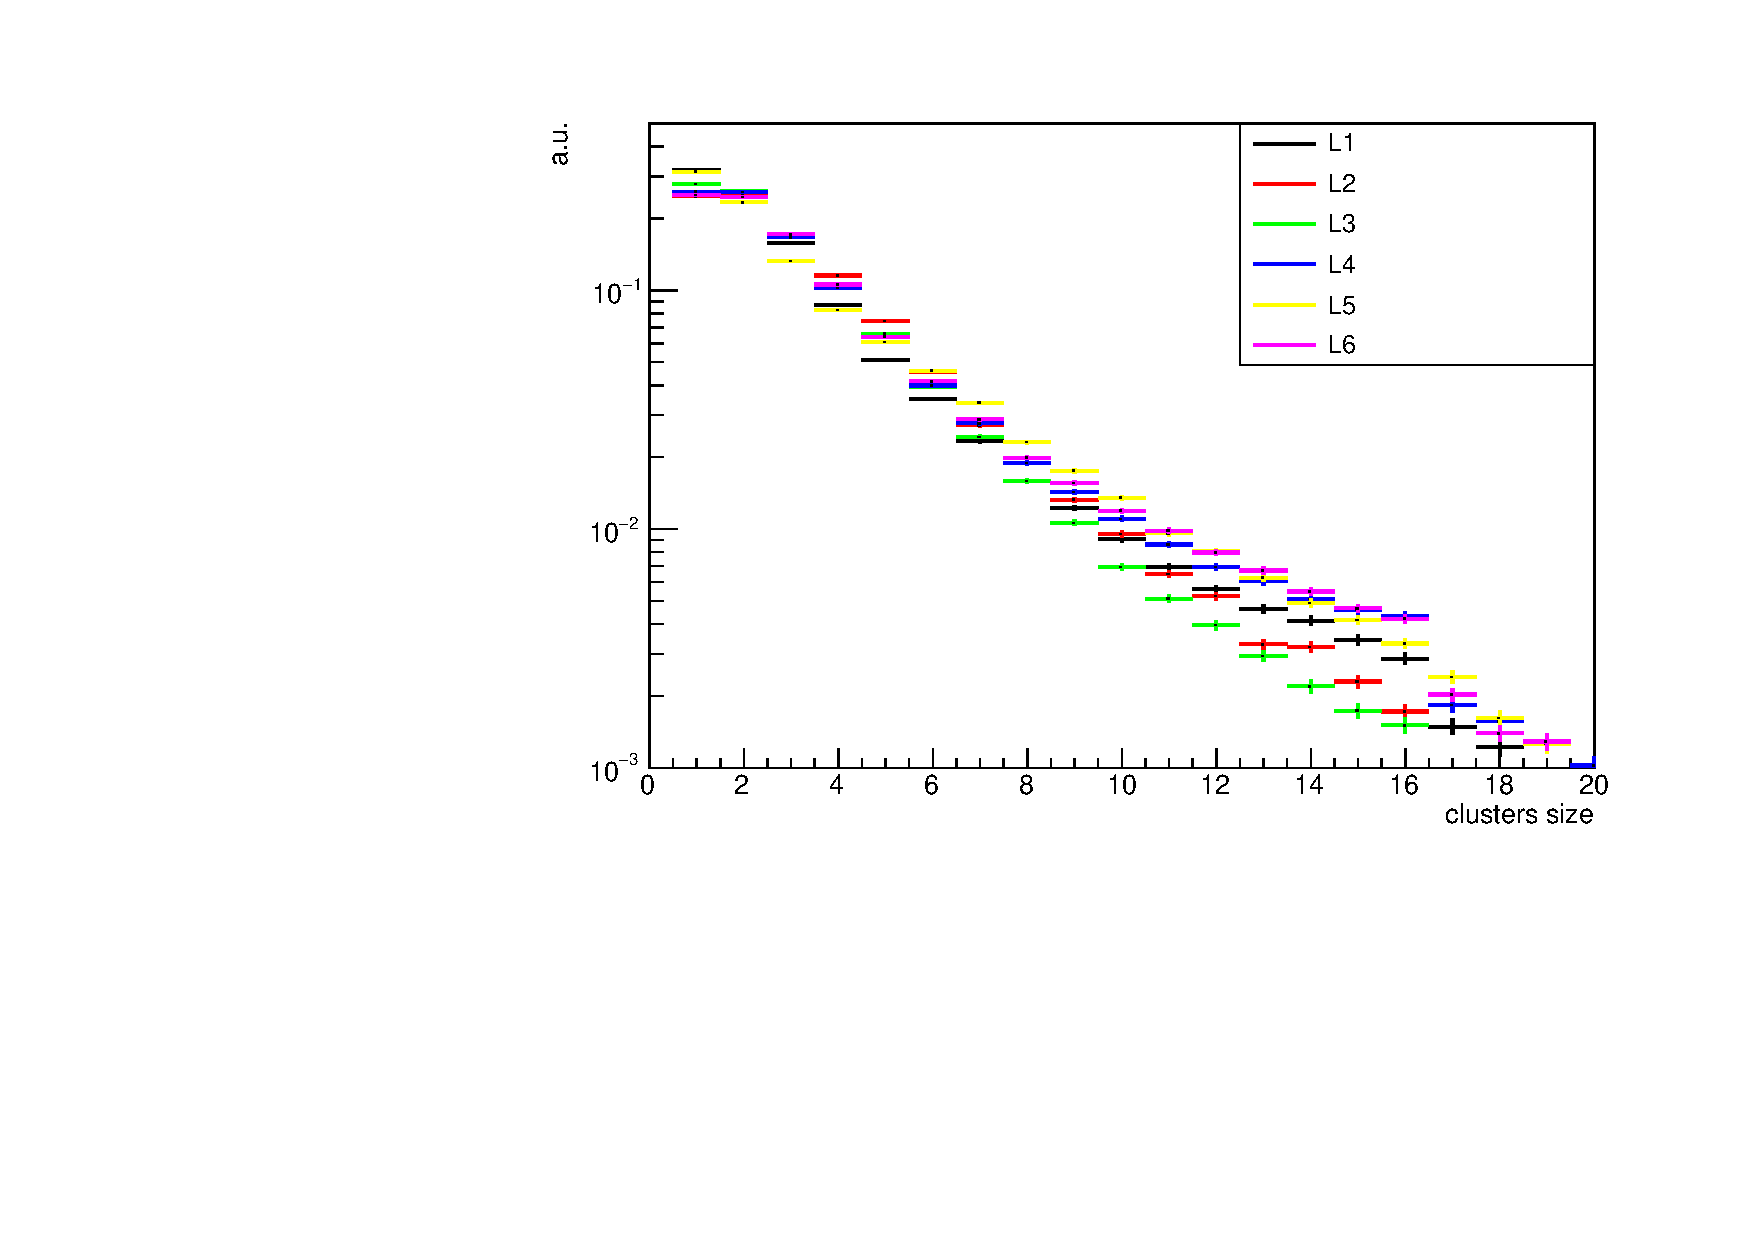
\includegraphics[width=.49\columnwidth,keepaspectratio]{images/beam_cls_size.pdf}
 \caption{(left) Number of clusters per event; (right) cluster size distribution. The beam current was 50~nA.}
 \label{fig:mm-beam_cls}
\end{figure}

Each MVT hit has an associated timestamp that can be used to compute the time difference of the signal with respect to the trigger. Consequently, a minimum time T$_{min}$ can be associated at each cluster as the minimum time among the hits that form the cluster. Figure~\ref{fig:mm-beam_cls_time} clearly shows that the clusters that have been associated with are reconstructed track have a similar T$_{min}$ distributions over the six BMT layers, \emph{i.e.} the clusters associated with a triggered physics event are strongly correlated in time. While the T$_{min}$ distributions of background clusters that are not associated to reconstructed tracks show a peak towards at very low values due to charged particles produced out of time with respect to the trigger.

\begin{figure}[htb]
 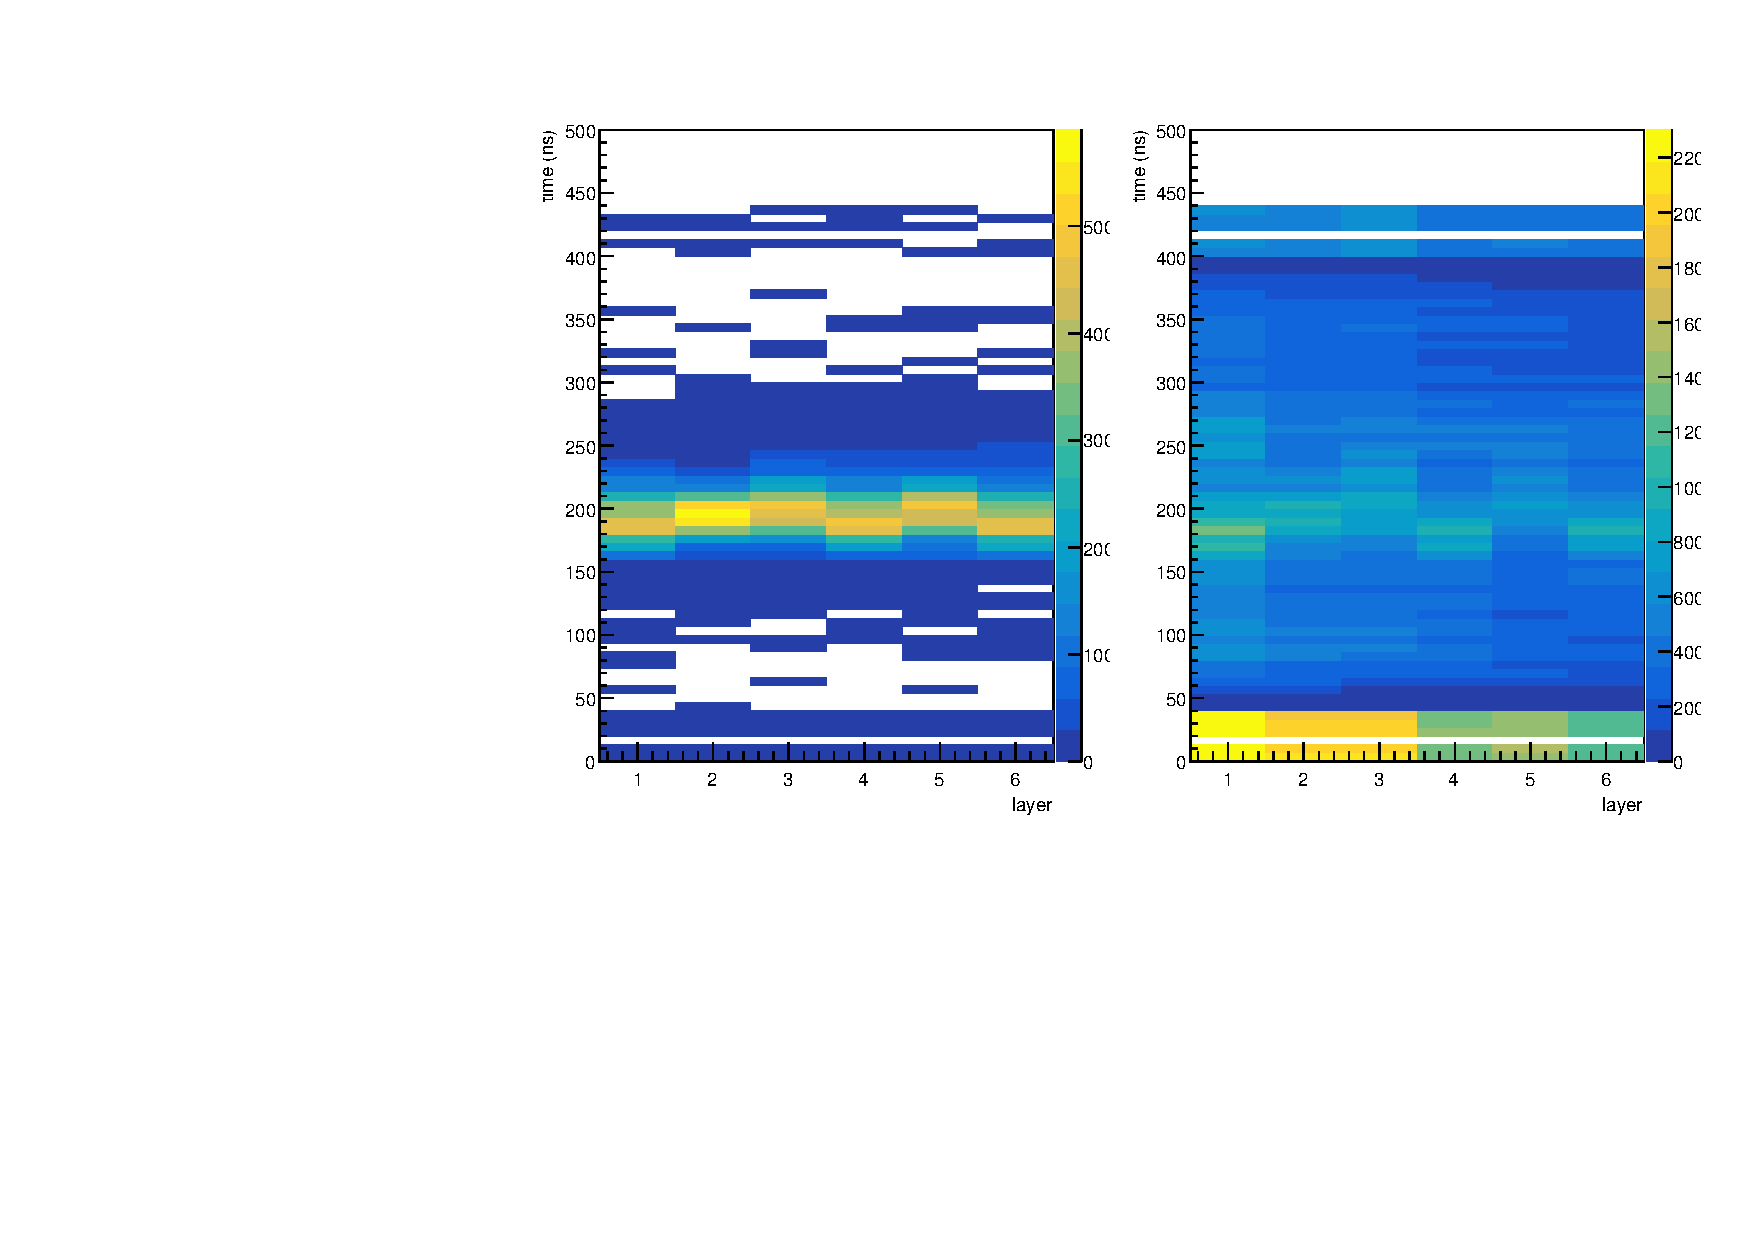
\includegraphics[width=\columnwidth,keepaspectratio]{images/align_cls_time.pdf}
 \caption{(left) Time distribution in the six BMT layers for clusters associated with a track; (right) Time distribution for clusters not associated with a reconstructed track.}
 \label{fig:mm-beam_cls_time}
\end{figure}


Special data taking periods with the empty target cell have been performed for calibration purposes as well as low luminosity runs with zero magnetic field for detector alignment studies. The standalone straight-track algorithm used for cosmic rays reconstruction has been adapted and extended to use SVT hits. Using preliminary alignment corrections for both SVT and BMT, a zero-field empty-target runs was reconstructed in SVT-standalone mode and CVT (\emph{i.e.} SVT$+$BMT) mode. As shown by Figure~\ref{fig:mm-zvertex}, the aluminum target walls are clearly visible in both reconstruction mode. It is possible to note that there is a significant improvement from $\sim$ 4.5~mm to 2.5~mm to the vertex position along the beam axis when the BMT information is used in the track reconstruction. Indeed the BMT-C tiles largely improve the polar angle of the particle with respect to the SVT-standalone mode. Concerning the azimuthal angle, the resolution of the BMT-Z tiles is not as good as the one of the SVT modules and they are further away from the beam axis. Therefore the improvement of the resolution on the azimuth angle of the track and related quantities like the (x,y) vertex coordinates is limited. On the other hand, BMT-Z tiles provide an essential redundancy for tracks that cross a limited number of SVT layers.

\begin{figure*}[htb]
 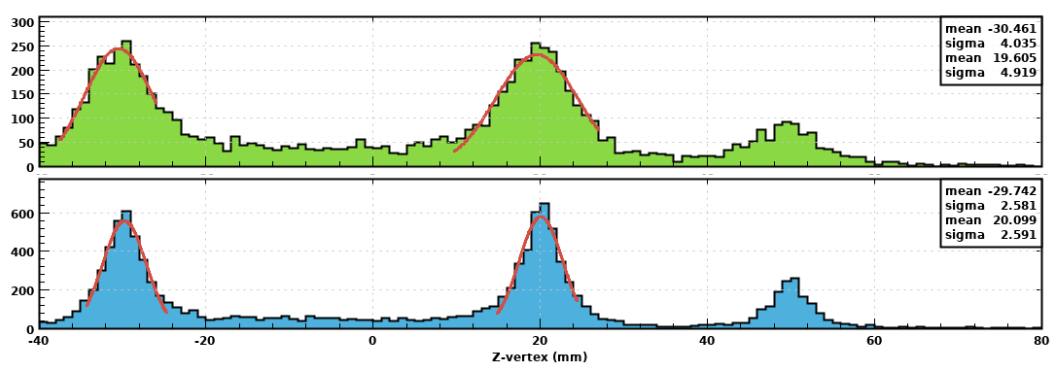
\includegraphics[width=2.0\columnwidth,keepaspectratio]{images/NIM_SVTvsCVT.png}
 \caption{Vertex position along the beam axis reconstructed with SVT-standalone reconstruction (top-green distribution) and CVT reconstruction (bottom-blue distribution) for an empty-target and no magnetic field run. The target walls are located at -30 and 20~mm with gaseous hydrogen in-between. At 50~mm, the scattering chamber cap is clearly visible. The improvement in the resolution from SVT to CVT reconstruction is due to the BMT-C tiles.}
 \label{fig:mm-zvertex}
\end{figure*}
